\section{開発の目的・ミッション定義}

\subsection{開発の目的}

平成26年度文部科学省宇宙航空科学技術推進委託費・宇宙科学研究拠点形成プログラム「革新的宇宙科学を切り拓く先進展開構造の研究・開発拠点形成」をきっかけに始めたプロジェクトを「ORIGAMI (ORganizatIon of research Group on Advanced deployable Membrane structures for Innovative space science) Project」と名付け,以下を目指す.
\begin{enumerate}
\item 多機能展開膜構造の宇宙実証と数値解析モデル高精度化
\item 継続的な展開構造物 宇宙実証のための「実験プラットフォーム」構築
\item 大学・企業が連携し宇宙実証を行う「研究・開発拠点」形成
\end{enumerate}

\subsection{ミッション定義}

上述3つの目的達成のためのパイロットプロジェクトとして,以下の3つのミッションを実施する衛星(3U CubeSat)を開発する.この衛星を,「OrigamiSat-1」と名付ける.なお,打ち上げ後にアマチュア無線通信に成功したことから,Fuji-OSCAR-98 (FO-98)の名称も付与された.したがって,「OrigamiSat-1/FO-98」あるいは「OrigamiSat-1 (FO-98)」を正式名称とする.
\begin{screen}
\noindent
\textbf{多機能膜展開ミッション:} 今後多様なアプリケーションへの発展を実現する目的で,開発者らが提案する多機能膜構造の展開・展張特性を軌道上で評価し,
(i) 膜構造の設計・検証手法の発展に寄与するデータを取得するとともに,(ii) 多様なユーザーへアピールする.\\
\noindent
\textbf{宇宙実証プラットフォーム開発ミッション:} 先進的展開構造の宇宙実証を容易にする目的で,主に大学・企業の研究者・技術者らに向けた宇宙実証プラットフォームを構築する.具体的には,(i) 市販衛星部品を利用した衛星開発を行いながら、(ii) 伸展マストを用いた軌道上撮影技術を獲得する.\\
\noindent
\textbf{アマチュア高速通信ミッション:} 衛星通信技術の発展と普及を目的に、アマチュア無線5.8GHz帯を用いた高速通信を実現する.
\end{screen}
\\

まず多機能膜展開ミッションでは,10cm × 10cm の筐体内から 1m × 1m サイズへと 2 次元方向に展開する多機能展開膜を軌道上で展開し、展開挙動・展張状態のデータを取得する。また、膜には薄膜デバイス(形状記憶合金アンテナ、太陽電池、球状太陽電池)を添付し、これらが機能することを検証する.

次に,宇宙実証プラットフォーム開発ミッションでは,今後の実証実験を容易にするため,(A) 販売機器を利用した衛星開発を行い,かつ (B) 伸展マストを用いた軌道上撮影技術を開発して,多機能展開膜の展開挙動および展張形状を計測する.

最後に,高速通信ミッションでは,アマチュア無線 5.84GHz 高速通信を用いた衛星通信を実現する.福岡工業大学が 2013 年に FITSAT-1 を用いて開発した衛星通信技術を実装・運用する.

\subsection{サクセスクライテリア}

OrigamiSat-1のサクセスクライテリアを,図\ref{2-1-1}に示す.
\begin{figure}[H]
	\centering
	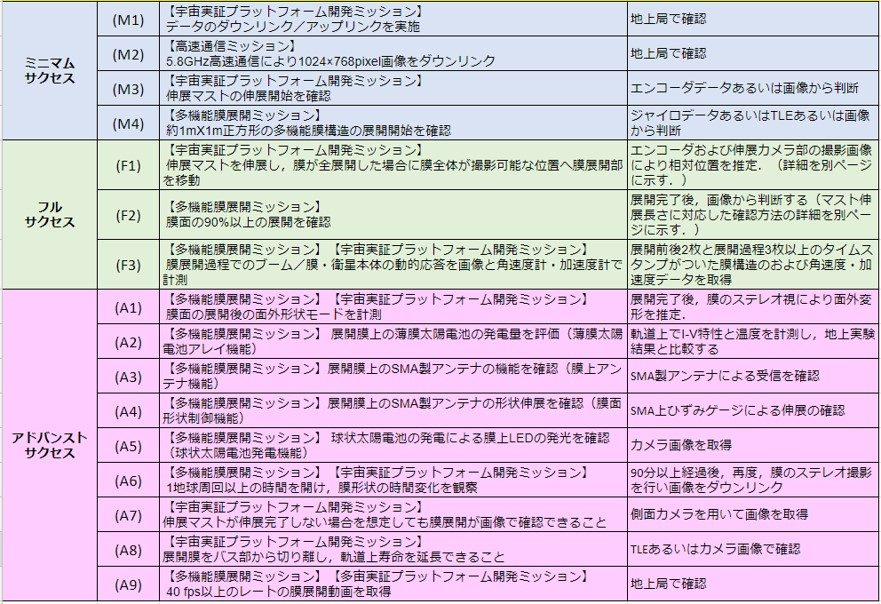
\includegraphics[width=\textwidth]{02/fig/2-1-1.jpg}
	\caption{3UキューブサットOrigamiSat-1 のサクセスクライテリア}
	\label{2-1-1}
\end{figure}

\subsection{ミッションシークエンス}
図\ref{fig2-1-2}に軌道投入後のミッションシークエンスを示す.本衛星はロケットより放出後,VHFおよびUHF用のモノポールアンテナを展開し,初期チェックアウトを実施する.その後,伸展カメラ部のマストを1m伸展することにより膜展開部がカメラの画角に入るよう調整し,多機能膜の展開・計測を行う.膜展開後は,膜形状の経時変化を定期的にカメラで計測する他,膜上の薄膜デバイスの機能検証を実施する.軌道高度が400km付近まで低下した後は軌道寿命を延長するため,伸展マストおよび膜展開部を切り離し2UサイズCubeSatとして,主に5.8GHz帯を用いた高速通信実験および,撮影データのダウンリンクを行う.
\begin{figure}[H]
	\centering
	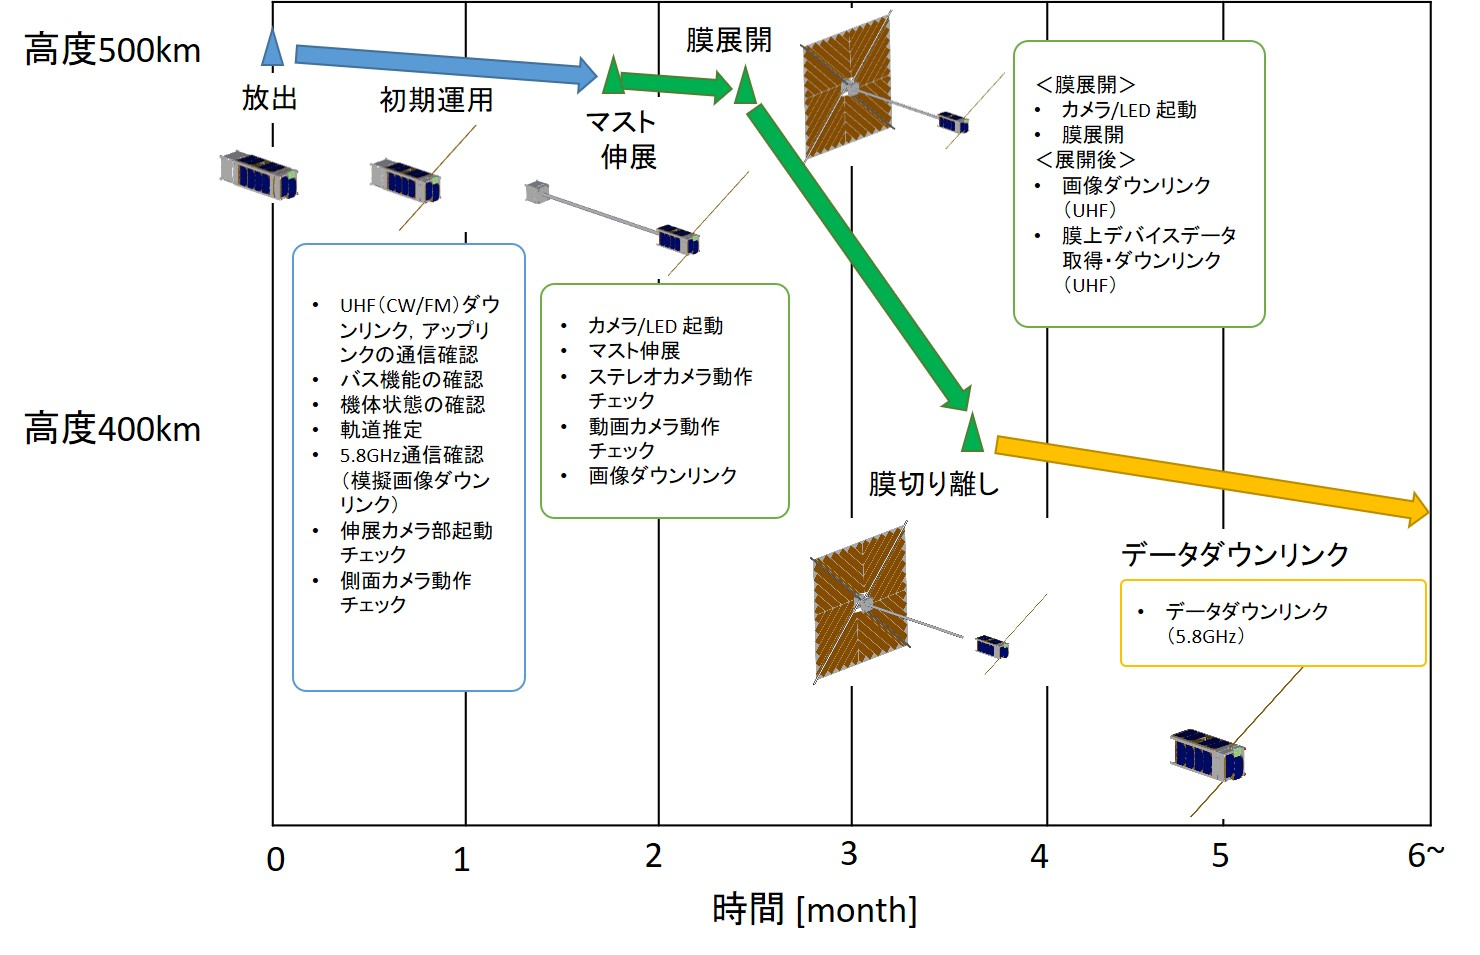
\includegraphics[width=\textwidth]{02/fig/2-1-2.jpg}
	\caption{3UキューブサットOrigamiSat-1 のミッションシークエンス可視化}
	\label{2-1-2}
\end{figure}
